\subsection{Prof. Dr. Nicola Spakowski}


\textbf{Main Research Interests}\\[-0.25cm]
\begin{enumerate}
\item[$\bullet$]	History of Modern and Contemporary China
\item[$\bullet$]	Historiography, History Teaching and the Popularization of History
\item[$\bullet$]	Feminism and Women Studies
\item[$\bullet$]	Internationalization, Globalization and Regionalization of China
\end{enumerate}


\vspace{0.6cm}
\textbf{Research Activities}\\[-0.25cm]

Nicola Spakowski in July 2006 completed her habilitation with a study of \textit{The military participation of women in the Chinese Communist revolution (1925-1949)} and a lecture titled \textit{From world to global history? Concepts of world history in China}. In 2006 she continued research on women soldiers in China, especially on aspects not addressed in the habilitation thesis (e.g. self-representations of women soldiers; women warriors in premodern China). 

\begin{}
  \begin{center}
    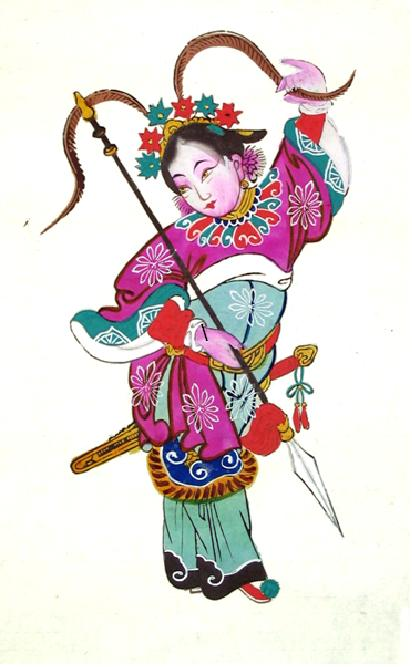
\includegraphics[width=0.45\textwidth]{./History/Spakowski.jpg}
    
		\caption{\itshape "A Chinese woman warrior as a door god"}%\label{fig:profxxx}
   \end{center}
\end{figure}\\
\vspace{0.3cm}
Recent research on \textit{Chinese feminism and women studies since the mid-1980s}, a project launched in the early 1990s, focused on the internationalization and indigenization of Chinese feminism. In particular, the introduction of the concept of "gender" into China and its adaptation to the Chinese context and alternatives to "gender" analysis in Chinese feminism were explored. Furthermore, Nicola Spakowski worked on a research proposal on \textit{The internationalization of the humanities and social sciences in the People's Republic of China} submitted to the DFG in June 2006. The project aims to identify the factors that shape internationalization processes in various fields of study. It focuses on two main questions: First, what are the channels, the institutional framework and the material basis for the internationalization of research in the social sciences and humanities in China? Second, what happens to a concept once it crosses national boundaries? Which meanings do categories and theories assume in discursive fields that are contested by a great variety of actors (Chinese mainland scholars, Chinese scholars from Hong Kong, Taiwan and the so-called "diaspora", Western scholars, the Chinese government, Western foundations etc.)? Finally, together with Marc Frey and Harald Fischer-Tin\'{e} she outlined a new project on \textit{Asianisms in the $20^{\rm th}$ century - Asian identity and interactions between nationalism, regionalism and global power structures}. The project explores Asia as a region and the idea of an Asian identity as a shaping force in economic, political, social and cultural interactions between Asian countries throughout the $20^{\rm th}$ century. This project will be submitted as a research proposal to the DFG in 2007.

\vspace{0.6cm}
\textbf{Other Professional Activities}\\[-0.25cm]
\begin{enumerate}
\item[$\bullet$] Member of the editorial advisory board of "Berliner China-Hefte"/"Chinese History and Society" 
\item[$\bullet$] Member of the steering committee of WAGNet (Women and gender in Chinese studies network)
\item[$\bullet$] Editor of WAGRev (Women and gender in Chinese studies review)
\item[$\bullet$] Organizer and chair of the panel "Through Many Lenses - Representations and Self-Representations of Women's Lives in 20th Century China", Biannual Conference of the European Association of Chinese Studies, Ljubljana, August 2006
\end{enumerate}
